%%% Modified template from:
% https://www.overleaf.com/read/qsdgxmhdwxxf
% http://www.aerialroboticscompetition.org/phpBB/viewtopic.php?t=302
\documentclass[12pt,letterpaper]{article}

% Supports accents
\usepackage[utf8]{inputenc}

\usepackage{graphicx,
	amssymb,
	titlesec,
	lipsum,
	lastpage,
	fancyhdr,
	titling}

% \includegraphics points to this folder by default
\graphicspath{ {images/} }

% Leading caps (first letter of word uppercase)
\usepackage{titlecaps}
\Addlcwords{to the of and or etc} % exclude

% References
\usepackage[style=numeric,backend=bibtex,backref=true,autolang=other,natbib]{biblatex} % http://goo.gl/wXN9T4
\bibliography{sections/references}

%% Figure caption formatting
\usepackage[labelfont=it,textfont=it,labelsep=period]{caption}
\usepackage[labelfont=it,textfont=it,labelsep=period]{subcaption}

%% Overall margins
\usepackage[margin=1in]{geometry}

%% Footer formatting
\fancyhf{}
\renewcommand{\headrulewidth}{0pt}
\pagestyle{fancy}
\cfoot{\textbf{\textsf{Page\ \thepage\ of \pageref{LastPage}}}}

%% Author list formatting
\newenvironment{nscenter}
{\parskip=0pt\par\nopagebreak\centering}
{\par\noindent\ignorespacesafterend}

\newcommand{\affiliatedauthor}[2]{
	\begin{nscenter}
		#1 \\ \textit{#2}
	\end{nscenter}
}

\newcommand{\affiliatedauthors}[1]{
	\begin{nscenter}
		#1
	\end{nscenter}
}
\newcommand{\affiliateduniversity}[1]{
	\begin{nscenter}
		\textit{#1}
	\end{nscenter}
}

%% Abstract formatting
\renewcommand{\abstractname}{ABSTRACT}

\renewenvironment{abstract}
{\vspace{-0.5ex}
	\small
	\begin{center}
		\bfseries \abstractname\vspace{-4ex}\vspace{0pt}
	\end{center}
	\list{}{
		\setlength{\leftmargin}{0.5in}
		\setlength{\rightmargin}{\leftmargin}
	}
	\item\relax}
{\endlist}

%% Section header formatting
\renewcommand\thesection{}
\renewcommand\thesubsection{}
\renewcommand\thesubsubsection{}
\titleformat{\section}{\normalfont\bfseries}{\thesection}{1em}{\MakeUppercase}
\titleformat{\subsection}{\normalfont\bfseries}{\thesubsection}{1em}{\titlecap}
\titleformat{\subsubsection}{\normalfont\itshape}{\thesubsubsection}{1em}{\titlecap}
\titlespacing*{\section}{0pt}{2ex}{-1.5ex}
\titlespacing*{\subsection}{0pt}{2ex}{-1.5ex}
\titlespacing*{\subsubsection}{0pt}{2ex}{-1.5ex}

%% Paragraph formatting (changing this messes with literally everything)
\setlength{\parindent}{0pt}
\setlength{\parskip}{2ex}

% Force figure to be centered
\makeatletter
\g@addto@macro\@floatboxreset\centering
\makeatother

%%%%%%%%%%%%%%%%%%%%%% ADD TITLE HERE %%%%%%%%%%%%%%%%%%%%%%
\title{Autonomous Quadrotor for the 201x IARC by Team Elikos}
%%%%%%%%%%%%%%%%%%%%%%%%%%%%%%%%%%%%%%%%%%%%%%%%%%%%%%%%%%%%

\begin{document}
	
	\begin{center}
		\textbf{\LARGE{\thetitle}}
	\end{center}
	
	%%%%%%%%%%%% SET AUTHOR NAMES AND AFFILIATIONS %%%%%%%%%%%%
	\affiliatedauthors{NAMES HERE}
	\affiliateduniversity{Team Elikos -- Polytechnique Montréal}
	%%%%%%%%%%%%%%%%%%%%%%%%%%%%%%%%%%%%%%%%%%%%%%%%%%%%%%%%%%%
	
	
	%%%%%%%%%%%%%%%%%%%%%%% ABSTRACT %%%%%%%%%%%%%%%%%%%%%%%
	\begin{abstract}
		The aim of this paper is to present team Elikos’ system design for a fully autonomous vehicle capable of solving IARC mission 7a. Using various sensors including GNC sensors, cameras, and lasers, the vehicle shall be able of robot interaction while avoiding obstacles, and present autonomous navigation capabilities based on computer vision and sensors analytics work. This paper emphasises the work of team Elikos for the 2016-2017 year.
	\end{abstract}
	%%%%%%%%%%%%%%%%%%%%%%%%%%%%%%%%%%%%%%%%%%%%%%%%%%%%%%%%
	
	%\clearpage
	
	%%%%%%%%%%%%%%%%%%%%%% MAIN TEXT %%%%%%%%%%%%%%%%%%%%%%
	
	%\section*{FIRST LEVEL HEADING}
	%\subsection*{Second Level Heading}
	%\subsubsection*{Third level heading}
	
	%\begin{figure}[h]
	%	\includegraphics[width=\textwidth]{}
	%	\vspace{-0.5cm}
	%	\caption{}
	%	\label{fig:}
	%\end{figure}
	
	
	% sections
	\section*{Introduction} \label{sec:intro}

\subsection*{Statement of the problem} \label{subsec:intro-problem}

Mission 7a of the International Aerial Robotics Competition involves a sheep and shepherd problem wherein the team’s aerial robot must herd terrestrial robots, hereinafter referred to as targets, by either triggering the top touch paddle or the bump sensor on their front side. The targets must be herded towards a green line within a 20x20-meter arena while dodging obstacle robots made of large PVC pipes roaming the arena in a circular motion. Mission completion is achieved when at least 4 targets, which have been interacted with, cross the green line.

\subsection*{Yearly milestones} \label{subsec:intro-milestones}

Team Elikos participated in the 2014 IARC edition with a Turnigy Talon V2 quadrotor frame modified to hold cameras and an embedded computer as well as wireless communication peripherals. The system was capable of relative position estimation through optical flow and was controlled by an automated ground station. 
In the 2015 IARC edition, our performance featured an aerial vehicle capable of target identification and pursuit, as well as an improved positioning system using SLAM and a completely revisited platform. 
Last year, Elikos presented a vehicle with an improved platform, target identification and pursuit, as well as a revisited positioning system. Some major work had also been put in the obstacle avoidance, interaction with grounds robots and functional artificial intelligence modules, although the IARC performance did not demonstrated all those functionalities.

Thereby, this year’s progress for team Elikos follows this work. As described in the present paper, we intend to demonstrate interaction with ground robots as well as stable and fully functional positioning system. Furthermore, the decision-making module of our autonomous vehicle has been greatly improved, thus connecting the different modules and bringing us one step closer to resolving the mission. Finally, some work have been put in the obstacle avoidance module, although we do not plan that the full integration with the rest of the operations will be accomplished by the time of the 2017 IARC edition.


\subsection*{Conceptual solution to solve the problem} \label{subsec:intro-solution}

This year’s solution for team Elikos has been developed based on challenges brought by the nature of Mission 7 itself as well as previous years learnings, as listed below:

\textbf{GPS-denied environment}: To compensate for the sterile environment as state by the competition rules - i.e. without externation navigation aids - the arena is filled with a 1-by-1-meter grid. As opposed to previous years, where we focused our work on the surrounding environment’s visual features (ceiling and walls), this year’s work is entirely based on the grid’s features, and entirely developed by our team. With this line of work, we were able to come with a solution specifically focused on the mission’s specifications, especially regarding the indoor aspect as well as the movements of our vehicle. Furthermore, we were able to test our solution both in virtual and physical environments almost identical to the competition’s. Our solution is described in the \textit{Stability Augmentation System} section.

It is important to mention that the position estimation from optical flow integration can quickly diverge from ground truth since every iteration adds small errors to the estimation. Thereby, this estimation, obtained by the PX4Flow Smart Camera, is fused with our visual solution, as explained in the \textit{Control System Architecture} section.

\textbf{Robots interaction}: The second biggest challenge comes from the interaction with the robots, requiring us to perform nearly aggressive vertical movements, and to approach the ground significantly. A direct consequence of this is that we lose all of our visual localization  when doing so, both from the grid’s features and from the optical flow - since the lens of the PX4Flow camera is fixed focus. Furthermore,  the ground effect can make the vehicle drift quickly with no means of it knowing so.

We tackled this problem by bypassing some modules of our usual pipeline in order to program those delicate maneuvers, as described in section \textit{Target Interaction}.

\textbf{High-level commands and strategy}: For the first time this year, we implemented a strategy module calculating the next robot we should interact with. The strategy is based on the position of the robots in relation to the green and red lines. The key aspect of this functionality lies in the ability to know - or estimate - the state of every ground robot. This challenge was tackled by the tracking module, as described in section \textit{Guidance, Navigation, and Control}.

\textbf{Overall hardware architecture}: This year’s solution is very similar to previous years regarding the hardware components. Indeed, we still use an onboard computer based on an Intel i5 processor and the Pixhawk open source flight controller, as those are high-performance off-the-shelf products. The Pixhawk offers an excellent development support and gives us the flexibility that we need. As mentioned before, we use the PX4Flow for optical flow position estimation, and the down-facing LIDAR-Lite laser for altitude measurement. Figure \ref{fig:intro-hardware} presents an overview of our vehicle’s hardware architecture.

This year's biggest alteration lies in the integration of mechanical switches under the landing gear to detect both interactions with ground robots and takeoff and landing operations.

\begin{figure}[h]
	\includegraphics[width=\textwidth]{overall_system_architecture.pdf}
	\vspace{-0.5cm}
	\caption{Overall hardware architecture.}
	\label{fig:intro-hardware}
\end{figure}

	\section*{Air vehicle} \label{sec:vehicle}

\subsection*{Propulsion and lift system} \label{subsec:vehicle-proplift}




\subsection*{Guidance, navigation, and control} \label{subsec:vehicle-gnc}

\subsubsection*{Stability augmentation system}



\subsubsection*{Navigation}



\subsubsection*{Target detection}



\subsubsection*{Target tracking}



\subsubsection*{Decision making}



\subsubsection*{Obstacle avoidance}



\subsubsection*{Target interaction}



\subsubsection*{Control system architecture}



\subsection*{Flight termination system} \label{subsec:vehicle-killswitch}


	\section*{Payload} \label{sec:payload}

\subsection*{Mechanical system} \label{subsec:payload-mechsystem}

Shown in Figure \ref{fig:payload-mech}, one of the main improvements made to the airframe is the addition of a new landing gear. This new component is essential, as the previous landing gear was composed of only four contact points which didn’t provide enough surface area to easily interact with the ground robots. Therefore, we added a carbon fiber sandwich panel with balsa under the structure. It greatly improves the quadcopter’s ability to physically interact with the ground robots, and adds another layer of protection for the components located under the quadcopter without adding much mass.

\begin{figure}[h]
	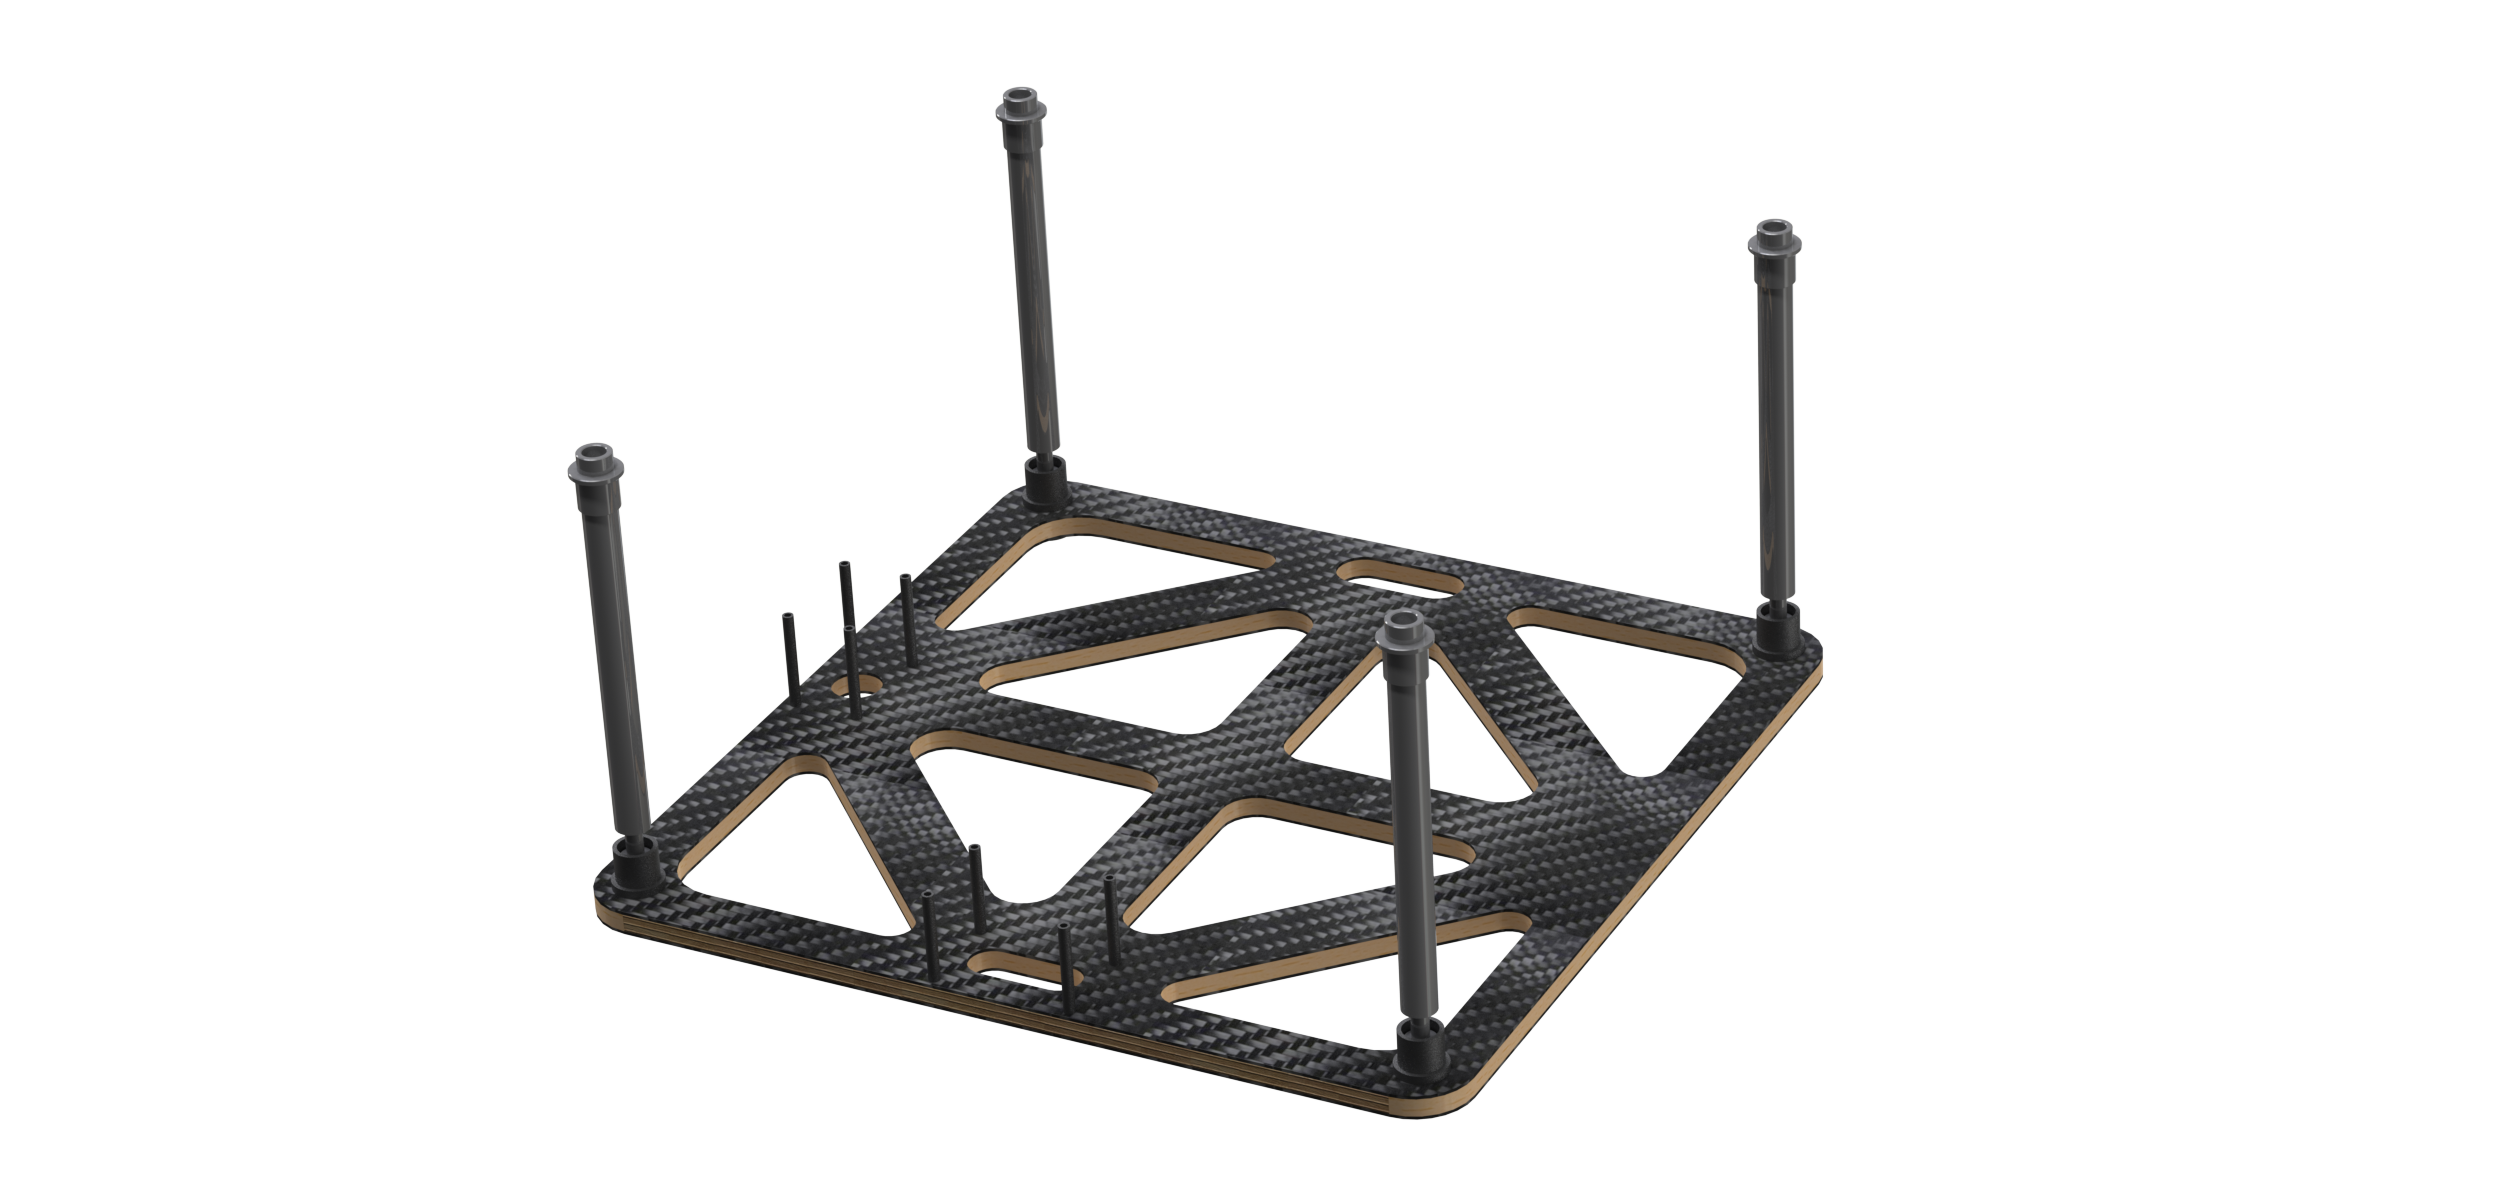
\includegraphics[width=0.6\textwidth]{render_belly.png}
	\vspace{-0.5cm}
	\caption{New landing gear for robot interaction.}
	\label{fig:payload-mech}
\end{figure}

\subsection*{Sensor suite} \label{subsec:payload-sensors}

\subsubsection*{GNC sensors}

The GNC sensor suite used for control is comprised of the Pixhawk’s inertial measurement unit (accelerometer, gyroscope, barometer, and compass), a PX4Flow optical flow camera, an external compass, and a LIDAR-Lite laser altitude sensor. The PX4 flight stack running on the Pixhawk is responsible to fuse all of this data, as explained in the \textit{Control System Architecture} section. 

\subsubsection*{Mission sensors}

The mission sensors include the four Intel RealSense 3D camera used for robot and obstacle detection and the Point Grey Firefly camera for visual localization. Their use is described in the \textit{Guidance, Navigation, and Control} section.

We have also integrated switches under the landing gear surface. With one switch under each landing leg, we can detect when legs touch the ground individually. This feedback is useful for autonomous landings or takeoffs. With another switch in the middle of the landing gear surface, we can detect physical interactions with ground robots. These switches are connected to an Arduino Nano, which is connected to the onboard computer through USB. The switch states are relayed to the computer through ROS messages with a \texttt{rosserial\_arduino} node and are then processed by the decision-making module.

\subsection*{Communications} \label{subsec:payload-comm}

Robot Operating System (ROS) is used to coordinate software communication between sensors, data processing, and decision-making modules. With its architecture, ROS allows for decentralized computation, which makes offboard processing possible through a Wi-Fi connection. However, offboard processing of the sensor data requires a high-bandwidth connection, but the wireless bands are cluttered by the teams running their own network. Therefore, during the IARC performance, the offboard computer is only used for monitoring through a 5~GHz network.

An RC receiver and a transmitter is used to activate offboard mode or for manual control when testing. A second RC receiver is used for the kill switch transmitter.

\subsection*{Power management system} \label{subsec:payload-power}

Our system is powered by two battery packs containing 4 lithium-ion polymer cells each. The three main systems of our vehicle are powered this way, that is the propulsion system, the flight controller and sensors system, and the onboard computer. The propulsion system is powered through the kill switch, as mentioned before. The Pixhawk is powered by a 5~V regulator (LM2678 from Texas Instruments). The onboard computer is powered through a 12~V DC power regulator (Murata UWE-12/10-Q12P-C).

	\section*{Operations} \label{sec:op}

\subsection*{Flight preparations} \label{subsec:op-prep}

There are many software and hardware pre- and post-flight checks in place. However, manual verifications are still required to ensure performance and safety during flights, since elements such as mechanical integrity cannot be automatically verified.

\subsubsection*{Pre-flight checklist}

The following is a checklist of elements and statuses that must be verified, at the very least, once before each extended flight session.

\vspace{-0.75cm}
\begin{enumerate} \itemsep -5pt
	\item Verify that the overall mechanical structure is undamaged and that the payload is securely mounted
	\item Verify that the propellers spin in the right directions and are properly tightened
	\item Verify that the Li-Po batteries are sufficiently charged ($ \approx 16.8 $~V) and well fastened
	\item Verify that the battery alarm is connected and functional
	\item Turn on and enable the kill switch transmitter
	\item Turn on the manual control transmitter
	\item Connect the batteries and power on the onboard computer, flight controller, and peripherals
	\item Verify that radio calibration and presets are correct
	\item Verify that the optical flow and computer vision cameras lenses are focused (and lens covers are removed)
	\item Calibrate inertial sensors (magnetometers, gyroscopes, accelerometers)
	\item Verify that telemetry and network communications are functional
\end{enumerate}

\subsubsection*{Post-flight checklist}

After each flight session or attempt, the following checks must be made.

\vspace{-0.75cm}
\begin{enumerate} \itemsep -5pt
	\item Properly terminate every process and data acquisition/logging
	\item Shut down the onboard computer and other peripherals
	\item Disconnect the batteries
	\item Turn off transmitters
	\item Verify that the battery levels are over the safety threshold and physically intact
	\item Verify that all component temperatures are within their normal operating temperatures
	\item Verify that every mount, propeller and screw is properly tightened (especially after a hard landing or a crash)
\end{enumerate}

\subsection*{Man/machine interface} \label{subsec:op-interface}

Prior to a flight, as mentioned in the \textit{Target Detection} section, a remote calibration tool for the cameras is used to adjust to the environment’s lighting.

In-flight, a SSH connection or a ROS remote connection allows us to monitor flight data over our Wi-Fi network. In case of emergency, the pilot’s transmitter offboard switch permits manual control at all time, and the kill switch’s dedicated transmitter cuts the power of all motors.

	\section*{Risk reduction} \label{sec:risk}

\subsection*{Vehicle status}\label{sec:risk-vehicle}

\subsubsection*{Shock/vibration isolation}

The sensors in the flight controller’s inertial measurement unit (IMU) are vulnerable to vibrations. It introduces noise in the sensor data which can ultimately lead to crashes. In order to minimize the impact of vibrations, the Pixhawk is mounted on a gel material with vibration isolation properties.

As for shock absorption, we’re using the same landing legs as the ones on the DJI Matrice 100. Since they contain both a spring and a damping mechanism, they’re useful for absorbing shocks resulting from reasonable drops of up to about 1~m. The landing legs are fixed to the frame with 3D-printed symmetrical parts pressed against the legs and fastened with screws.

\subsubsection*{EMI/RFI solutions}

The EM noise generated by the propulsion system can be troublesome to the flight controller’s internal compass. For this reason, we use an external magnetometer mounted on the very top, as far away from the power circuitry as possible.

\subsection*{Safety} \label{subsec:risk-safety}

The main physical safety feature is a 3D-printed prop guard. It is designed to counter shocks towards the inside of the quadcopter. Identical parts are fixed under every motor using the same mounting holes. Each part offers 90-degree protection around a motor. To get an all-around, complete 360-degree protection, we added rigid carbon fiber rods between prop guards. These rods are also useful for mounting sensors.

\subsection*{Modeling and simulation} \label{subsec:risk-modelsim}

The SolidWorks software is used for the mechanical design of our custom parts. It’s also useful for the integration of all other components and to optimize usable space for sensor mounting.

\begin{figure}[h]
	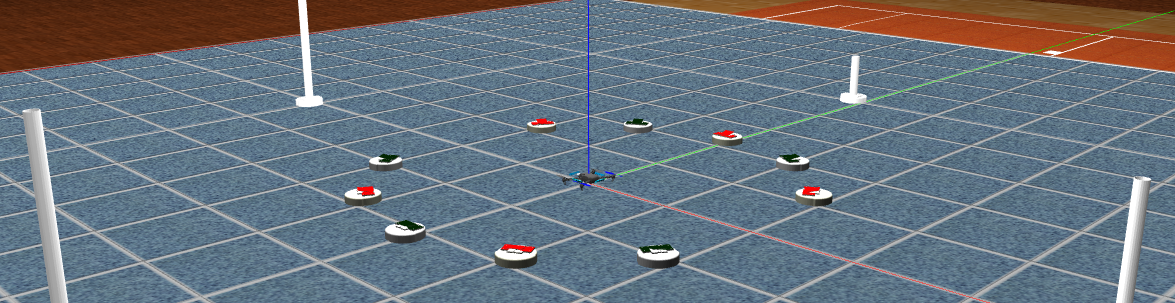
\includegraphics[width=\textwidth]{gazebo_2.png}
	\vspace{-0.5cm}
	\caption{Mission 7 simulation in Gazebo.}
	\label{fig:model-gazebo}
\end{figure}

As a part of our software development process, we use the Gazebo simulator \cite{koenig2004design} to reproduce the 7th mission’s arena and to model the physics of a quadcopter controlled by a software in the loop (SITL) version of the Pixhawk controller. We added most of the quadcopter sensors, like the 2D and 3D cameras. Our simulation also includes the floor pattern used at the competition and the 3D models of the targets and obstacles as illustrated on figure \ref{fig:model-gazebo}.

\subsection*{Testing} \label{subsec:risk-test}

\textbf{Motion capture:} Polytechnique’s Electrical Engineering Department acquired a VICON Motion Capture, allowing us to fly indoor with an external navigation system. We were then able to test all of our other modules, including target identification and pursuit, high-level strategy, and threat avoidance in an environment similar to the competition’s, without the localization module being finalized.

\textbf{Competition environment:} Last year, we acquired a 5x5 vinyl grid surface similar to the one used at the American Venue. This helped us reproduce the environment of the competition, allowing us to test our different modules more deeply than with the simulation.

\textbf{Ground and obstacle robots:} To test target detection and tracking, we have built ground and obstacle robots according to the reference instructions. However, for the control and programming of the Create 2 robots, we have decided not to use the reference Arduino setup. Instead, we mounted a Raspberry Pi 3 model B powered by a USB power bank on each robot. It runs a ROS node for the ground and obstacle robots behavior implementation and uses a driver package for serial communication \cite{roscreateautonomy}. All robots are connected via Wi-Fi to our network. Therefore, we can control and send commands to the robots with the computer used for monitoring. We can also easily remotely control the robots with a game controller.

	\section*{Conclusion}


	
	\printbibliography
	
\end{document}